%%This is a very basic article template.
%%There is just one section and two subsections.
\documentclass[a4paper, ngerman]{scrartcl}

\usepackage[T1]{fontenc}
\usepackage[utf8]{inputenc}
\usepackage[ngerman]{babel}
\usepackage{lmodern}
\usepackage{amsmath}
\usepackage{amsfonts}
\usepackage{hyperref}
\usepackage{graphicx}
\usepackage{paralist}
\usepackage[none]{hyphenat}
\usepackage{wrapfig}

\sloppy



\hypersetup{
pdfborder = {0 0 0},
urlbordercolor = {0 0 0},
colorlinks = true,
linkcolor = black,
citecolor = black,
filecolor = black,
urlcolor  = black
}

\title{Software-Challenge 2014 - Sixpack}
\subtitle{Spielregeln}



%% Variablen
\newcommand{\SpielFelderAnzahl}{\emph{256}}
\newcommand{\KartenAnzahl}{\emph{KartenAnzahl}}
\newcommand{\PiratenAnzahl}{\emph{6}}
\newcommand{\EmptyPlainPage}{\newpage\thispagestyle{plain}\ \newpage}
\newcommand{\RundenAnzahl}{\emph{15}}

\begin{document}
\parindent0px
\maketitle

\begin{figure}[h]
	\centering
	%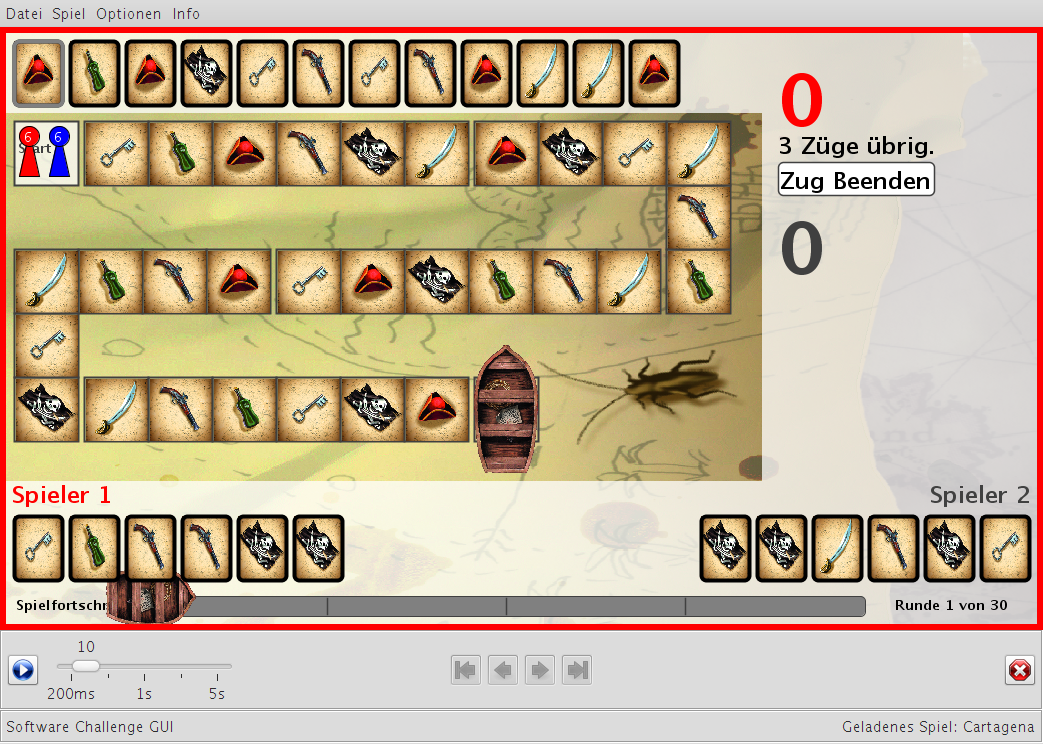
\includegraphics[width=\linewidth]{bilder/Uebersicht.png}
\end{figure}
\vspace*{\fill}

\newpage
\tableofcontents
\newpage

\section{Einführung}
In dieser Anleitung werden die Elemente und Regeln des Spiels \emph{Sixpack}
der Software-Challenge 2014 erläutert.\\
In dem Spiel versuchen zwei Spieler durch geschicktes Anlegen von Spielsteinen auf einem Spielbrett möglichst viele Punkte zu erlangen.

\section{Spielmaterial}
	\subsection{Das Spielbrett}
Das Spielbrett wird durch insgesamt \SpielFelderAnzahl\ Spielfeldern, welche in einer 16x16 Matrix angeordnet sind, gebildet. Die Nummerierung der Spielfelder beginnt dabei, wie in der Informatik üblich, bei 0. Jedes Spielfeld besitzt einen eindeutigen Index der sich aus x und y Komponente zusammensetzt, nach dem Schema (x,y). Das Spielfeld ganz links oben besitzt demnach den Index (0,0) (siehe Abbildung ~\ref{fig:Spielfeld}).\\

\begin{figure}[h] \centering 
	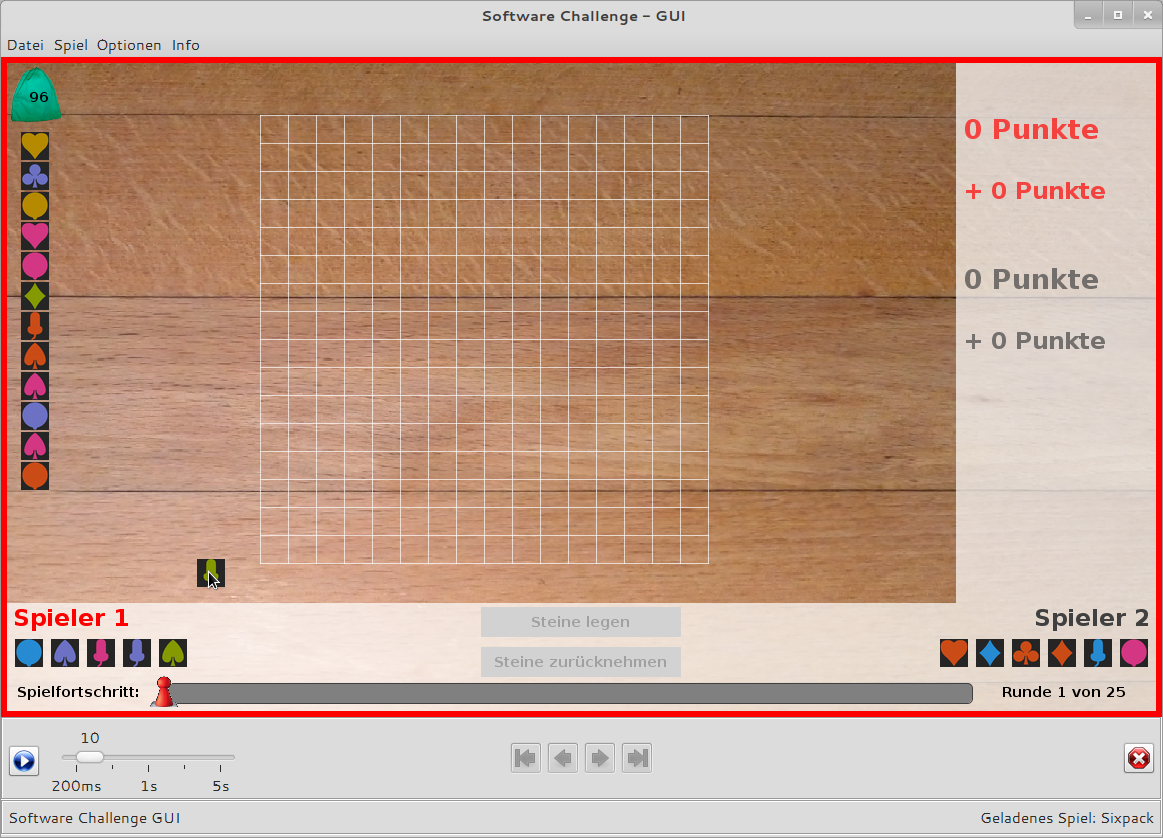
\includegraphics[scale = 0.3]{images/Spielbrett}
	\caption{Das Spielbrett.}
	\label{fig:Spielfeld}
\end{figure}

\subsection{Die Spielsteine}
Ein Spielstein besitzt eine von sechs möglichen Farben und eine von sechs möglichen Formen. Es existieren demnach 36 verschiedene Farb/Form Kombinationen (siehe siehe Abbildung ~\ref{fig:Spielsteine}).\\

\begin{figure}[h] \centering 
	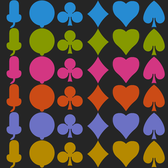
\includegraphics[scale = 0.8]{images/Spielsteine}
	\caption{Alle möglichen Farbe/Form Kombinationen der Spielsteine}
	\label{fig:Spielsteine}
\end{figure}

Von jeder Kombination gibt es genau drei Steine im Spiel, also insgesamt 108 Spielsteine. Alle Spielsteine werden zu Beginn des Spiels gemischt und im Spielsteinbeutel abgelegt. Die nächsten 12 Spielsteine, welche aus dem Beutel gezogen werden können, werden unterhalb des Beutels angezeigt. Die Nummer auf dem Beutel gibt die Anzahl der sich noch im Beutel befindenden Spielsteine an. Hierbei ist zu beachten, dass damit die Gesamtanzahl der Spielstein im Vorrat gemeint ist. Sowohl die nicht einsehbaren, als auch die schon sichtbaren Spielsteine unterhalb des Beutels.\\

\begin{figure}[h] \centering 
	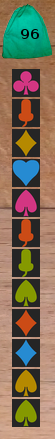
\includegraphics[scale = 0.7]{images/Vorratsbeutel}
	\caption{Der Vorratsbeutel}
	\label{fig:Vorratsbeutel}
\end{figure}
Jeder Spieler besitzt zu Beginn und am Ende seines Zuges immer genau 6 Steine in seinem Vorrat, wobei auch der Vorrat des gegnerischen Spieler eingesehen werden kann.\\




	

\section{Spielablauf}		
	Es beginnt der rote Spieler. Jeder Spieler hat in seinem Zug zwei verschiedene Möglichkeiten. Entweder er legt einen oder mehrere Spielsteine auf dem Spielbrett aus, oder er tauscht 1-6 seiner Spielsteine gegen neue ein.	
	
\subsection{Spielsteine auslegen}

	 
\subsection{Spielsteine tauschen}




\subsection{Spezialfall: Keine Züge möglich}

	
\subsection{Punkteverteilung}
	
\section{Ende des Spiels}

	Hat ein Spieler alle seine Piraten im Zielfeld, so gewinnt dieser. Schafft dies
	keiner der beiden Spieler innerhalb der \RundenAnzahl\ Runden, so
	gewinnt der Spieler mit den meisten Punkten.
	
\section{Die graphische Benutzeroberfläche}
\subsection{Übersicht der graphischen Benutzeroberfläche}
	In Abbildung~\ref{fig:GUI} ist ein Überblick der graphischen Benutzeroberfläche
	zu sehen. Die markanten Spielelemente sind mit \emph{a-e} gekennzeichnet.
	
	 \begin{figure}[h!]
		\centering		
		%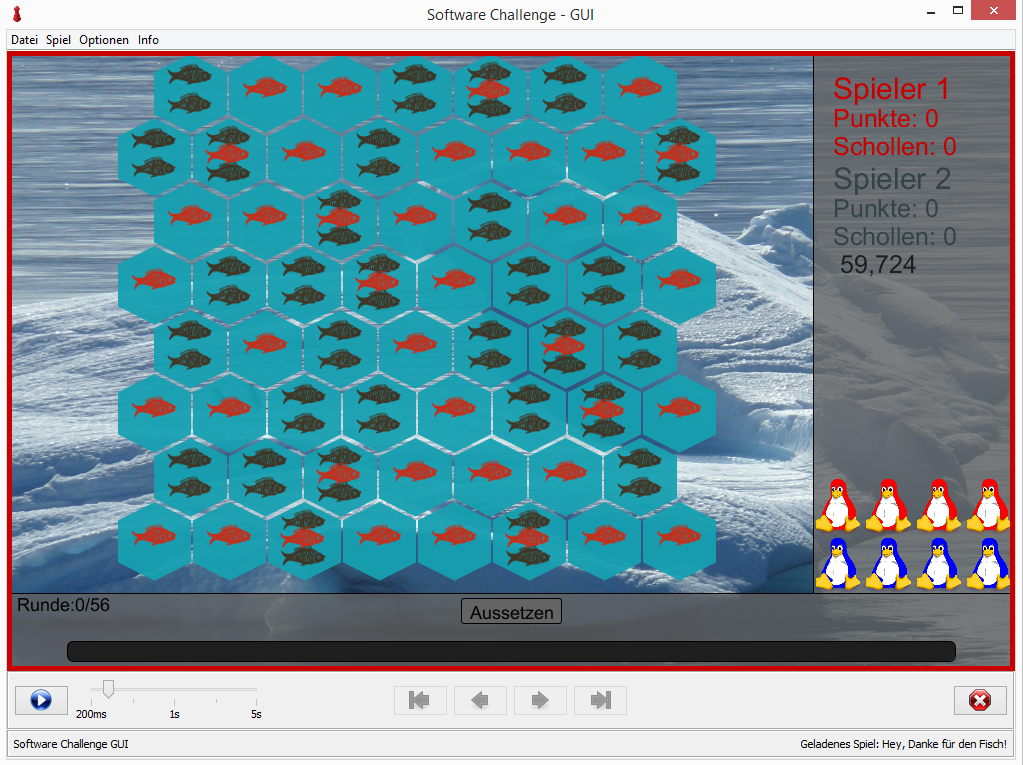
\includegraphics[scale = 0.3]{bilder/gui}
		\caption{Überblick der GUI}
		\label{fig:GUI}
	\end{figure}
	
\begin{compactenum}[a)] \item Die nächsten ziehbaren Karten. Die Erste befindet
sich links.
\item Das Spielbrett \item Punkteanzeige, Anzeige der verbleibenden Züge und
Button, um einen Zug vorzeitig zu beenden. Die Punkte des roten Spielers sind
oben, die des blauen Spielers unten. Die Punkte des inaktiven Spielers sind
jeweils immer grau.
\item Die Karten von Spieler 1. Neu dazugekommene Karten werden immer Richtung
Bildmitte positioniert.
\item Spielfortschrittsanzeige
	\end{compactenum}
	
\subsection{Das Einstellungsmenü}
	 \begin{figure}[h]
		\centering
		%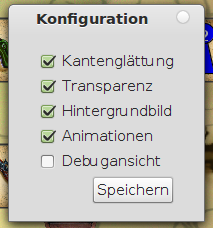
\includegraphics[scale=0.5]{bilder/configuration}
		\caption{Das Einstellungsmenü}
		\label{fig:Configuration}
	\end{figure}
	
	Ein Einstellungsmenü mit Darstellungsoptionen lässt
sich über die Leertaste anzeigen. Dazu muss das
Spielfeld den Tastaturfokus haben (erforderlichenfalls
vorher Mausklick auf das Spielfeld). Es stehen dort
folgende Einstellungen zur Verfügung:

\textbf{Kantenglättung} und \textbf{Transparenz} verbessern die Optik des
Spiels, sind aber rechenintensiv. Auf sehr langsamen Rechnern sollten sie daher
deaktiviert werden. \textbf{Hintergrundbild} ist zwar weniger rechenintensiv,
kann aber auch aus Gründen der Übersichtlichkeit deaktiviert werden.\\
\textbf{Animationen} legt fest, ob die Bewegungen der Spielsteine in
Wiederholungen und bei Computerspielern animiert werden sollen.\\
Die \textbf{Debugansicht} verkleinert die Punkteanzeige in der Seitenleiste
etwas und zeigt unterhalb Debug-Hilfestellungen zu einzelnen Zügen an. Diese
Hilfestellungen sind Texte, die ein Spielclient einem Zug beifügen kann, den er
an den Spielserver sendet.
	
\end{document}
